%%%%%%%%%%%%%%%%%%%%%%%%%%%%%%%%%%%%%%%%%
% Structured General Purpose Assignment
% LaTeX Template
%
% This template has been downloaded from:
% http://www.latextemplates.com
%
% Original author:
% Ted Pavlic (http://www.tedpavlic.com)
%
% Note:
% The \lipsum[#] commands throughout this template generate dummy text
% to fill the template out. These commands should all be removed when 
% writing assignment content.
%
%%%%%%%%%%%%%%%%%%%%%%%%%%%%%%%%%%%%%%%%%

%----------------------------------------------------------------------------------------
% PACKAGES AND OTHER DOCUMENT CONFIGURATIONS
%----------------------------------------------------------------------------------------

\documentclass{article}

\usepackage{fancyhdr} % Required for custom headers
\usepackage{lastpage} % Required to determine the last page for the footer
\usepackage{extramarks} % Required for headers and footers
\usepackage{graphicx} % Required to insert images
\usepackage{lipsum} % Used for inserting dummy 'Lorem ipsum' text into the template
\usepackage{amsmath, amsfonts, bm, physics}
\usepackage{xcolor}
\usepackage{listings}
\usepackage{hyperref}
\usepackage[toc,page]{appendix}

\lstset{
    %numbers=left,
    stepnumber=1,    
    firstnumber=1,
    numberfirstline=true,
    basicstyle=\ttfamily,
    keywordstyle=\color{blue}\ttfamily,
    stringstyle=\color{red}\ttfamily,
    commentstyle=\color{green}\ttfamily,
    breaklines=true,
}

% Margins
\topmargin=-0.45in
\evensidemargin=0in
\oddsidemargin=0in
\textwidth=6.5in
\textheight=9.0in
\headsep=0.25in 

\linespread{1.1} % Line spacing

% Set up the header and footer
\pagestyle{fancy}
\lhead{\hmwkAuthorName} % Top left header
\chead{\hmwkClass\ (\hmwkClassInstructor\ \hmwkClassTime): \hmwkTitle} % Top center header
\rhead{\firstxmark} % Top right header
\lfoot{\lastxmark} % Bottom left footer
\cfoot{} % Bottom center footer
\rfoot{Page\ \thepage\ of\ \pageref{LastPage}} % Bottom right footer
\renewcommand\headrulewidth{0.4pt} % Size of the header rule
\renewcommand\footrulewidth{0.4pt} % Size of the footer rule

\setlength\parindent{0pt} % Removes all indentation from paragraphs

%----------------------------------------------------------------------------------------
% DOCUMENT STRUCTURE COMMANDS
% Skip this unless you know what you're doing
%----------------------------------------------------------------------------------------

% Header and footer for when a page split occurs within a problem environment
\newcommand{\enterProblemHeader}[1]{
  \nobreak\extramarks{#1}{#1 continued on next page\ldots}\nobreak
  \nobreak\extramarks{#1 (continued)}{#1 continued on next page\ldots}\nobreak
}

% Header and footer for when a page split occurs between problem environments
\newcommand{\exitProblemHeader}[1]{
  \nobreak\extramarks{#1 (continued)}{#1 continued on next page\ldots}\nobreak
  \nobreak\extramarks{#1}{}\nobreak
}

\setcounter{secnumdepth}{0} % Removes default section numbers
\newcounter{homeworkProblemCounter} % Creates a counter to keep track of the number of problems

\newcommand{\homeworkProblemName}{}
\newenvironment{homeworkProblem}[1][]{ % Makes a new environment called homeworkProblem which takes 1 argument (custom name) but the default is "Problem #"
  \stepcounter{homeworkProblemCounter} % Increase counter for number of
% problems
  \setcounter{homeworkSectionctr}{0}
  %\renewcommand{\homeworkProblemName}{#1} % Assign \homeworkProblemName the
% name of the problem
  \section{\arabic{homeworkProblemCounter}. #1} %
  % Make a section in the document with the
% custom problem count
  \enterProblemHeader{\homeworkProblemName} % Header and footer within the
% environment
}{
  \exitProblemHeader{\homeworkProblemName} % Header and footer after the
% environment
}

\newcommand{\problemAnswer}[1]{ % Defines the problem answer command with the content as the only argument
  \noindent\textbf{\emph{Answer: }}#1 % Just put a keyword Answer in
  % bold/italic at the beginning
}

%\newcommand{\homeworkSectionName}{}
%\newenvironment{homeworkSection}[1]{ % New environment for sections within
% homework problems, takes 1 argument - the name of the section
%  \renewcommand{\homeworkSectionName}{#1} % Assign \homeworkSectionName to the
% name of the section from the environment argument
%  \subsection{\homeworkSectionName} % Make a subsection with the custom name
% of the subsection
%  \enterProblemHeader{\homeworkProblemName\ [\homeworkSectionName]} % Header
% and footer within the environment
%}{
%  \enterProblemHeader{\homeworkProblemName} % Header and footer after the
% environment
%}

\newcounter{homeworkSectionctr}
\newenvironment{homeworkSection}{
  \medskip\noindent%         create a vertical offset to previous material
  \refstepcounter{homeworkSectionctr}% increment the environment's counter
  \textbf{(\alph{homeworkSectionctr})\ }% or \textbf,.
}

\newtheorem{theorem}{Theorem}[homeworkProblemCounter]
\newtheorem{lemma}[theorem]{Lemma}
\newtheorem{proposition}[theorem]{Proposition}
\newtheorem{corollary}[theorem]{Corollary}

\newenvironment{proof}[1][Proof]{
  \begin{trivlist}
    \item[\hskip \labelsep {\bfseries #1}]}{
  \end{trivlist}
}
\newenvironment{definition}[1][Definition]{
  \begin{trivlist}
    \item[\hskip \labelsep {\bfseries #1}]}{
  \end{trivlist}
}

\newenvironment{example}[1][Example]{
  \begin{trivlist}
    \item[\hskip \labelsep {\bfseries #1}]}{
  \end{trivlist}
}
    
\newenvironment{remark}[1][Remark]{
  \begin{trivlist}
    \item[\hskip \labelsep {\bfseries #1}]}{
  \end{trivlist}
}

\newcommand{\qed}{
  \nobreak \ifvmode \relax \else
  \ifdim\lastskip<1.5em \hskip-\lastskip
  \hskip1.5em plus0em minus0.5em \fi \nobreak
  \vrule height0.75em width0.5em depth0.25em\fi
}

\lstset{
  frame=single,
  breaklines=true,
  postbreak=\raisebox{0ex}[0ex][0ex]{\ensuremath{\color{red}\hookrightarrow\space}}
}
   
%----------------------------------------------------------------------------------------
% NAME AND CLASS SECTION
%----------------------------------------------------------------------------------------

\newcommand{\hmwkTitle}{Assignment\ \#2} % Assignment title
\newcommand{\hmwkDueDate}{Monday, April\ 11,\ 2016} % Due date
\newcommand{\hmwkClass}{STA\ 208} % Course/class
\newcommand{\hmwkClassTime}{MW 12:00 - 2:00 P.M.} % Class/lecture time
\newcommand{\hmwkClassInstructor}{Prof. James Sharpnack} % Teacher/lecturer
\newcommand{\hmwkAuthorName}{Wenhao Wu} % Your name

%----------------------------------------------------------------------------------------
% TITLE PAGE
%----------------------------------------------------------------------------------------

\title{
  \vspace{2in}
  \textmd{\textbf{\hmwkClass:\ \hmwkTitle}}\\
  \normalsize\vspace{0.1in}\small{Due\ on\ \hmwkDueDate}\\
  \vspace{0.1in}\large{\textit{\hmwkClassInstructor\ \hmwkClassTime}}
  \vspace{3in}
}

\author{\textbf{\hmwkAuthorName}}
\date{} % Insert date here if you want it to appear below your name

%----------------------------------------------------------------------------------------

\begin{document}

  \maketitle
  
  %----------------------------------------------------------------------------------------
  % TABLE OF CONTENTS
  %----------------------------------------------------------------------------------------
  
  %\setcounter{tocdepth}{1} % Uncomment this line if you don't want subsections listed in the ToC
  
  \newpage
  \tableofcontents
  \newpage
  
  %----------------------------------------------------------------------------------------
  % PROBLEM 1
  %----------------------------------------------------------------------------------------
  \begin{homeworkProblem}
    The following losses are used as surrogate losses for large margin
    classification. Demonstrate if they are convex or not, and follow the
    instructions.
    
    \begin{homeworkSection}
      exponential loss: $\phi(x)=e^{-x}$
      \vspace{10pt}
      
      \problemAnswer{
        Since $d^2\phi(x)/dx^2 = e^{-x} > 0$, this function is convex.
      }
    \end{homeworkSection}
    
    \begin{homeworkSection}
      truncated quadratic loss: $\phi(x)=(\max\{1-x, 0\})^2$
      \vspace{10pt}
      
      \problemAnswer{
        We can rewrite $\phi(x)=(\max\{1-x, 0\})^2$
        \begin{align}
          \phi(x)= \left\{
            \begin{array}{ll}
              (1-x)^2 & x < 1,\\
              0 & \mbox{otherwise.}
            \end{array}
          \right.
        \end{align}
        Then the convexity of $\phi(x)$ can be proved by the definition
        \begin{itemize}
          \item $\forall x_1 < 1, x_2 < 1$ or $\forall x_1\geq 1, x_2\geq 1$,
          since both $f(x) = (1-x)^2$ and $g(x)=0$ are convex functions, we have
          \begin{align}
            \phi(tx_1 + (1 - t)x_2) \leq t\phi(x_1) + (1 - t)\phi(x_2)
          \end{align}
          $\forall t\in [0,1]$.
          \item $\forall x_1 < 1, x_2 \geq 1$, since $\phi(x)$ is monotonically
          decreasing,
          \begin{align}
            \phi(tx_1 + (1 - t)x_2) \leq \phi(tx_1) = t\phi(x_1) + (1 -
            t)\phi(x_2)
          \end{align}
        \end{itemize}
        Therefore $\phi(x)$ is convex.
      }
      
    \end{homeworkSection}
    
    \begin{homeworkSection}
      hinge loss: $\phi(x) = \max\{1 - x, 0\}$
      \vspace{10pt}
      
      \problemAnswer{
        Since both $f(x) = 1-x$ and $g(x)=0$ are convex functions, $(\max\{1-x,
        0\})$, $\phi(x)$ is also convex.
      }
    \end{homeworkSection}
    
    \begin{homeworkSection}
      sigmoid loss: $\phi(x) = 1 - \tanh(\kappa x)$, for fixed $\kappa > 0$
      \vspace{10pt}
      
      \problemAnswer{
        Since 
        \begin{subequations}
          \begin{align}
            \dv{\phi}{x} & = \frac{-4\kappa e^{2\kappa x}}{(1 + e^{2\kappa x})}
            = \kappa\phi(x)(\phi(x) - 2) \\
            \dv[2]{\phi}{x} & = 2\kappa^2\phi(x)(\phi(x) - 2)(\phi(x) - 1)
          \end{align}
        \end{subequations}
        when $x<0$, $d^2\phi/dx^2 < 0$, therefore $\phi(x)$ is not convex.
      }
    \end{homeworkSection}
    
    \begin{homeworkSection}
      Plot these as a function of $x$.
      \vspace{10pt}
      
      \problemAnswer{
        \begin{figure}[h]
          \centering
          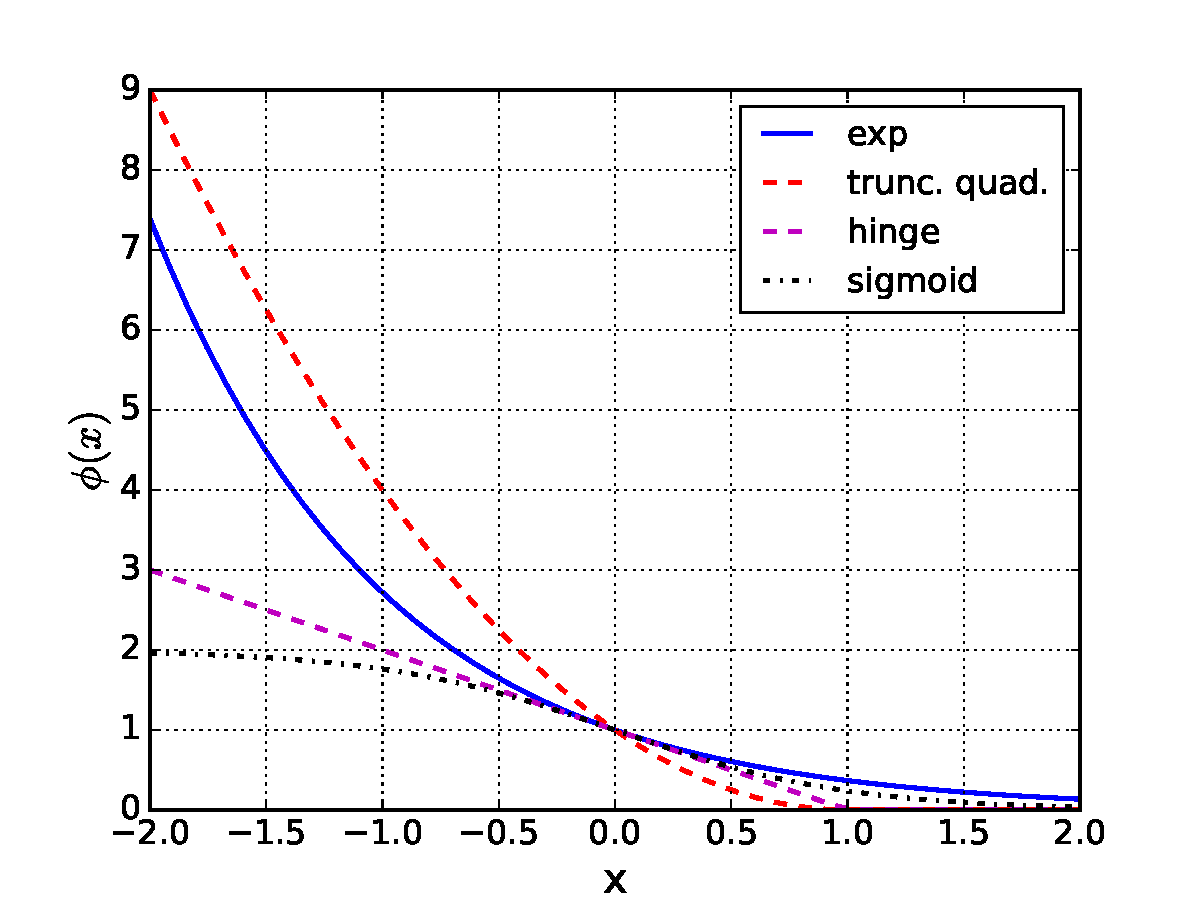
\includegraphics[width=3.5in]{figs/loss.pdf}
          \caption{Comparison of different loss functions.}
          \label{fig:loss}
        \end{figure}
      }
\begin{lstlisting}[language=Python]
import numpy as np
import matplotlib.pyplot as plt
import matplotlib as mpl
%matplotlib qt

x = np.linspace(-2, 2, num=50)
kappa = 1 # The parameter for the sigmoid loss

axis_font = {'size':'20'}
mpl.rcParams['xtick.labelsize'] = 16
mpl.rcParams['ytick.labelsize'] = 16

plt.plot(x, np.exp(-x), 'b-', linewidth=2, label="exp")
plt.plot(x, (1-x).clip(0) ** 2, 'r--', linewidth=2, label="trunc. quad.")
plt.plot(x, (1-x).clip(0), 'm--', linewidth=2, label="hinge")
plt.plot(x, 1 - np.tanh(kappa * x), 'k-.', linewidth=2, label="sigmoid")
plt.legend(prop={'size':16})
plt.grid()
plt.xlabel('x', **axis_font)
plt.ylabel('$\phi(x)$', **axis_font)
\end{lstlisting}
    \end{homeworkSection}
    
    (This problem is due to notes of Larry Wasserman.)
  \end{homeworkProblem}
  %\clearpage
  
  %----------------------------------------------------------------------------------------
  % PROBLEM 2
  %----------------------------------------------------------------------------------------
  \begin{homeworkProblem}
    Consider the least-squares problem with $n$ $p$-dimensional covariates,
    $\{\mathbf{x}_i, y_i\}_{i=1}^n \subset \mathbb{R}^p \times \mathbb{R}$. We
    would like to fit the following linear model, $\hat{y}(\mathbf{x}) =
    \mathbf{x}^T\bm{\beta}$. Also, suppose that there are coefficients $C_+
    \subset \{1, \ldots , p\}$ such that for all $j \in C_+$ we require that
    $\beta_j \geq 0$, $j\in C_+$, and another set $C_- \subset \{1, \ldots,
    p\}$, such that $\beta_j \leq 0$, $j \in C_-$ (assume that $C_+$ and $C_-$
    are non-overlapping). Suppose that $\mathbf{X}^T\mathbf{X}$ is invertible.
      
    Such examples occur in insurance applications: the cost of a given insurance
    policy is based on a model for the amount of money a customer will cost the
    company, and each covariate is a variable specific to the customer (such as
    gender, age, credit history, etc.). It looks bad for the company if the
    insurance policy is more expensive for a customer that has an older account
    with the company than a newer account, when everything else is held fixed.
    Let $x_{i,j} = 1\{\mbox{customer $i$ is has had a policy for more than 2
    years}\}$, then $\beta_j \geq 0$ is necessary for this property to hold.

    \begin{homeworkSection}
      Write the constrained optimization for the empirical risk minimization
      with the constraints.
      \vspace{10pt}
      
      \problemAnswer{
        \begin{subequations}
          \begin{align}
            & \min_{\bm{\beta}}\|\mathbf{y} - \mathbf{X}\bm{\beta}\|_2^2 \\
            \mbox{s.t. } & \beta_j \geq 0,\, j\in C_+ \\
            & \beta_j \leq 0,\, j\in C_-
          \end{align}
        \end{subequations}
      }
    \end{homeworkSection}
    
    \begin{homeworkSection}
      Derive the dual for the optimization as a function of dual parameters.
      \vspace{10pt}
      
      \problemAnswer{
        The Lagrangian is given by
        \begin{align}
          L(\bm{\beta},\bm{\lambda}) = \frac{1}{2}\|\mathbf{y} -
          \mathbf{X}\bm{\beta}\|_2^2 + \bm{\beta}^T\bm{\lambda}
        \end{align}
        where $\lambda_j \geq 0$ for $j\in C_-$ and $\lambda_j \leq 0$ for $j\in
        C_+$.
        Set derivative to 0, we have
        \begin{align}
          \pdv{L}{\bm{\beta}} = -\mathbf{X}^T(\mathbf{y} - \mathbf{X}\bm{\beta})
          + \bm{\lambda} = 0
          \label{eq:lagrangian}
        \end{align}
        therefore
        \begin{align}
          \hat{\bm{\beta}} = (\mathbf{X}^T\mathbf{X})^{-1}
          (\mathbf{X}^T\mathbf{y} - \bm{\lambda})
          \label{eq:beta}
        \end{align}
        substitute back into~\eqref{eq:lagrangian}, the dual function is
        \begin{align}
          l(\bm{\lambda}) = \frac{1}{2}\mathbf{y}^T\mathbf{y} - \frac{1}{2}
          (\mathbf{X}^T\mathbf{y} - \bm{\lambda})^T
          (\mathbf{X}^T\mathbf{X})^{-1} (\mathbf{X}^T\mathbf{y} - \bm{\lambda})
        \end{align}
      }
    \end{homeworkSection}
      
    \begin{homeworkSection}
      Write the KKT conditions and remark on the implication of the
      complementary slackness condition.
      \vspace{10pt}
      
      \problemAnswer{
        The KKT conditions are
        \begin{subequations}
          \begin{align}
            & -\mathbf{X}^T(\mathbf{y} - \mathbf{X}\bm{\beta})
            + \bm{\lambda} = 0;\;(\mbox{stationarity}) \\
            & \beta_j \geq 0,\, j\in C_+;\; \beta_j \leq 0,\, j\in
            C_-;\;(\mbox{primal feasibility}) \\
            & \lambda_j \leq 0,\, j\in C_+;\; \lambda_j \geq 0,\, j\in
            C_-;\;(\mbox{dual feasibility})\\
            & \lambda_j \beta_j = 0.\;(\mbox{complementary slackness})
          \end{align}
        \end{subequations}
        The complementary slackness condition implies that, if
        $\lambda_j\not=0$ we must have $\beta_j=0$, and if $\beta_j\not=0$ we
        must have $\lambda_j=0$.
      }
    \end{homeworkSection}
    
  \end{homeworkProblem}
  
  %----------------------------------------------------------------------------------------
  % PROBLEM 3
  %----------------------------------------------------------------------------------------
  \begin{homeworkProblem}
    Look at the dataset which can be found here: \url{https://archive.ics.uci.edu/ml/datasets/Blood+Transfusion+Service+Center}
      
    \begin{homeworkSection}
      You will predict the final column in the dataset, which is an indicator if
      the person has made a blood donation. Form three different kernel
      functions and $n\times n$ kernel matrices of $K_{i,j} = k(\mathbf{x}_i,
      \mathbf{x}_j)$ that you think might be appropriate. You may use 2
      different built in kernels, but must define one yourself.
      \vspace{10pt}
      
      \problemAnswer{
        We will use two-built in kernels from scikit-learn, namely the linear
        kernel and the radial basis function kernel. We will also use the
        Epanechnikov kernel function
        \begin{align}
          K(x, x') = D\left(\frac{|x - x'|}{\lambda} \right)
        \end{align}
        where
        \begin{align}
          D(t) = \left\{
            \begin{array}{ll}
              \frac{3}{4}(1-t^2) & |t|<1, \\
              0 & \mbox{otherwise.}
            \end{array}
          \right.
        \end{align}
      }
    \end{homeworkSection}
    
    \begin{homeworkSection}
      Apply kernel SVMs and $k$-nearest neighbors (where the distance is $d(i,
      j) = k(\mathbf{x}_i, \mathbf{x}_i) + k(\mathbf{x}_j, \mathbf{x}_j) -
      2k(\mathbf{x}_i, \mathbf{x}_j))$ with each of the 3 kernels.
      \vspace{10pt}
      
      \problemAnswer{
        See next section.
      }
    \end{homeworkSection}
      
    \begin{homeworkSection}
      Tune any parameters based on what you have learned about validation, and
      compare these methods with test errors (there are 6 different methods to
      compare, kNN and SVM with each kernel).
      \vspace{10pt}
      
      \problemAnswer{
        We split the dataset into a 25\% test set and a 75\% training+validation
        set. The parameters of the rbf kernel and the Epanechnikov kernel are
        tuned based on a Stratified ShuffleSplit cross validation, where the
        test\_size is set to $1/3$ of the training+validation dataset (25\% of
        the original dataset) with 5 iterations.
        
        The range of tuning parameters are set as follows. For the support
        vector classifier, we take $\log C=\mbox{range}(-4,4)$. For the
        k-nearest neighbor classifier we take $k = \mbox{range}(1,15)$. For
        the rbf kernel, we take $\log \gamma=\mbox{range}(-4,4)$. For the
        Epanechnikov kernel, we take bandwidth $\log l=\mbox{range}(-3,3)$.
        
        The tuning and testing results of the 6 tuned classifiers shown in
        Table.~\ref{table:comparison}. These results suggest that all the
        classifiers perform almost equally badly, as a trivial classifier always
        output 0 would achieve almost the same score over the given dataset.
        
        \begin{table}[!t]
          \renewcommand{\arraystretch}{1.3}
          \caption{Comparison of different classifiers.}
          \label{table:comparison}
          \centering
          \begin{tabular}{c|ccc}
            \hline
            Classifier & Optimal parameters & Training score & Test score
            \\
            \hline
            SVC+Linear & $C=10^4$ & 0.7754 & 0.7326 \\
            SVC+RBF & $\gamma=10^{-2}$, $C=10^2$ & 0.7840 & 0.7433 \\
            SVC+Epanechnikov & $l=10^2$, $C=10^3$ & 0.7743 & 0.7326 \\
            KNN+Linear & $k=2$ & 0.7786 & 0.7380 \\
            KNN+RBF & $k=2$, $\gamma=10^{-4}$ & 0.7797 & 0.7380 \\
            KNN+Epanechnikov & $k=2$, $l=10$ & 0.7797 & 0.7380 \\
            \hline
          \end{tabular}
        \end{table}
      }
    \end{homeworkSection}
\begin{lstlisting}[language=Python]
import pandas as pd
import numpy as np
import timeit
import sys

from sklearn import preprocessing, neighbors
from sklearn.svm import SVC
from sklearn.neighbors import KNeighborsClassifier
from sklearn.cross_validation import train_test_split, StratifiedShuffleSplit
from sklearn.grid_search import GridSearchCV
from sklearn.base import BaseEstimator, TransformerMixin
from sklearn.pipeline import Pipeline

df = pd.read_csv('transfusion.data') # Import the datafile
X = preprocessing.scale(df.values[:, :4].astype("float64")) # The predictors, standardized
y = df.values[:, 4] # The responses
X_train, X_test, y_train, y_test = train_test_split(X, y, test_size=0.25) # Set aside 25% of the data for test
print("{0} is 0, {1} is 1".format(1 - sum(y) / len(y), sum(y) / len(y)))

cv = StratifiedShuffleSplit(y_train, n_iter=5, test_size=1/3, random_state=42) # Generate the cross validation labels

C_range = np.logspace(-4, 4, 9) # Range of Parameter C for all 3 svcs
k_range = np.arange(1, 15) # Range of parameter n_neighbors for all 3 knncs

gamma_range = np.logspace(-4, 4, 9) #  Range of parameter gamma for rbf kernel
l_range = np.logspace(-3, 3, 7) # Range of parameter l for Epanechnikov kernel

classifiers = dict() # The set of classifiers
params_grid = dict() # The set of cross validation parameters for each classifier

# The svm classifier with linear kernel
classifiers["svc_linear"] = SVC(kernel='linear')
params_grid["svc_linear"] = dict(C=C_range)

# The svm classifier with rbf kernel
classifiers["svc_rbf"] = SVC(kernel='rbf')
params_grid["svc_rbf"] = dict(gamma=gamma_range, C=C_range)

# The svm classifier with user defined Epanechnikov kernel
def epa(X, Y, l=1.0):
    """ Epanechnikov kernel with bandwidth parameter
    return a n_row_X-by-n-row_Y matrix
    """
    n_sample_X = len(X)
    n_sample_Y = len(Y)
    t = np.empty([n_sample_X, n_sample_Y], dtype="float64")
    for i in range(n_sample_X):
        for j in range(n_sample_Y):
            t[i, j] = np.linalg.norm(X[i] - Y[j]) / l
    
    return 3 / 4  * (1 - t ** 2) * (abs(t) < 1)

class EpaKernel(BaseEstimator, TransformerMixin):
    def __init__(self, l=1.0):
        super(EpaKernel, self).__init__()
        self.l = l

    def transform(self, X):
        return epa(X, self.X_train_, l=self.l)

    def fit(self, X, y=None, **fit_params):
        self.X_train_ = X
        return self
    
classifiers["svc_epa"] = Pipeline([('epa', EpaKernel()),('svm', SVC()),])
params_grid["svc_epa"] = dict([('epa__l', l_range), ('svm__kernel', ['precomputed']), ('svm__C', C_range),])

# The knn classifier with linear kernel
classifiers["knnc_linear"] = neighbors.KNeighborsClassifier()
params_grid["knnc_linear"] = dict(n_neighbors=k_range)

# The knn classifier with rbf kernel
def kernel_rbf(x, y, gamma):
    return np.exp(-gamma * np.linalg.norm(x-y)  ** 2)

def dist_rbf(x, y, gamma):
    return kernel_rbf(x, x, gamma) + kernel_rbf(y, y, gamma) - 2 * kernel_rbf(x, y, gamma)

classifiers["knnc_rbf"] = neighbors.KNeighborsClassifier(metric=dist_rbf)
params_grid["knnc_rbf"] = dict(metric_params=[{'gamma': gamma} for gamma in gamma_range], n_neighbors=k_range)

# The knn classifier with user defined Epanechnikov kernel
def kernel_epa(x, y, l):
    t = np.linalg.norm(x - y) / l
    return 3 / 4  * (1 - t ** 2) if abs(t) < 1 else 0.0

def dist_epa(x, y, l):
    return kernel_epa(x, x, l) + kernel_epa(y, y, l) - 2 * kernel_epa(x, y, l)

classifiers["knnc_epa"]  = neighbors.KNeighborsClassifier(metric=dist_epa)
params_grid["knnc_epa"] = dict(metric_params=[{'l': l} for l in l_range], n_neighbors=k_range)

for classifier in classifiers.keys():
    start_time = timeit.default_timer()
    
    print("Tuning {0}...".format(classifier))
    
    grid = GridSearchCV(classifiers[classifier], param_grid=params_grid[classifier], cv=cv, verbose=0, n_jobs=4)
    grid.fit(X_train, y_train)
    
    print(" - The best parameters are {0} with a score of {1}".format(grid.best_params_, grid.best_score_))
    print(" - The score on the test set is {0}".format(grid.score(X_test, y_test)))
    print(" - Elapsed time is {0}".format(timeit.default_timer() - start_time))
    sys.stdout.flush()
\end{lstlisting}
  \end{homeworkProblem}
  
  %\newpage
  %\begin{appendices} 
  %\end{appendices}
  %\bibliographystyle{unsrt}
  %\bibliography{refs}
  
  %----------------------------------------------------------------------------------------

\end{document}